\documentclass{article}
\usepackage{tikz}
\usepackage{tkz-graph}
\usetikzlibrary{shapes.symbols,positioning,shapes.multipart}
\newcommand{\measurepoint}[2]{%
  \pgfextractx{\dimen0}{#2}\pgfextracty{\dimen2}{#2}%
  \typeout{LAYOUT-POINT #1: x=\the\dimen0, y=\the\dimen2}}
\begin{document}
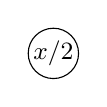
\begin{tikzpicture}
  \node[draw,circle,font=\small,inner xsep=0pt,inner ysep=1pt] (compact) {$x/2$};
  \measurepoint{compact-east}{\pgfpointanchor{compact}{east}}
  \measurepoint{compact-west}{\pgfpointanchor{compact}{west}}
\end{tikzpicture}
\begin{tikzpicture}
  \node[anchor=west,xshift=.2] (a) at (1,1) {$a$};
  \node[anchor=north,yshift=-.1] (b) at (2,2) {$b$};
  \measurepoint{a}{\pgfpointanchor{a}{center}}
  \measurepoint{b}{\pgfpointanchor{b}{center}}
\end{tikzpicture}
\begin{tikzpicture}[scale=1.2]
  \draw (0,1cm) -- node[anchor=west] (height) {$h$} (0,1.5cm);
  \measurepoint{height}{\pgfpointanchor{height}{center}}
\end{tikzpicture}
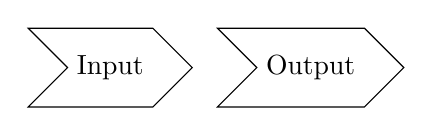
\begin{tikzpicture}[node distance=8mm]
  \node[signal,signal from=west,signal to=east,minimum width=2cm,minimum height=1cm,draw] (input) {Input};
  \node[signal,signal from=west,signal to=east,minimum width=2cm,minimum height=1cm,draw,right=of input] (output) {Output};
  \measurepoint{input-center}{\pgfpointanchor{input}{center}}
  \measurepoint{input-east}{\pgfpointanchor{input}{east}}
  \measurepoint{output-center}{\pgfpointanchor{output}{center}}
  \measurepoint{output-west}{\pgfpointanchor{output}{west}}
\end{tikzpicture}
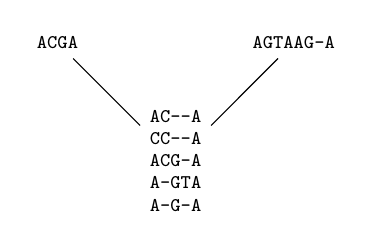
\begin{tikzpicture}[font=\tt\scriptsize,grow=up,level 1/.style={sibling distance=30mm}]
  \node[align=center](root){AC{-}{-}A\\CC{-}{-}A\\ACG-A\\A-GTA\\A-G-A}
    child{node{AGTA\\AG-A}}
    child{node{ACGA}};
  \measurepoint{tree-start}{\pgfpointshapeborder{root}{\pgfpointanchor{root-1}{center}}}
  \measurepoint{tree-end}{\pgfpointshapeborder{root-1}{\pgfpointanchor{root}{center}}}
\end{tikzpicture}

\begin{tikzpicture}[scale=.8,every node/.style={scale=.7},font=\tt]
  \GraphInit[vstyle=Normal]\SetGraphUnit{2.5}
  \tikzset{VertexStyle/.append style={fill}}
  \Vertex{AT}\EA(AT){TG}
  \measurepoint{vertex-east}{\pgfpointanchor{AT}{east}}
  \measurepoint{vertex-west}{\pgfpointanchor{AT}{west}}
\end{tikzpicture}
\tikzset{font=\tt,every picture/.style={thick},node/.style={rectangle split,rectangle split horizontal,rectangle split parts=#1,draw,rectangle split empty part width=1.5}}
\begin{tikzpicture}
  \node[node=13] (A) {\nodepart{one}\tiny False\nodepart{two}5\nodepart{three}\nodepart{four}-3\nodepart{five}\nodepart{six}0\nodepart{seven}\nodepart{eight}4\nodepart{nine}\nodepart{ten}17\nodepart{eleven}\nodepart{twelve}42\nodepart{thirteen}};
  \measurepoint{split-east}{\pgfpointanchor{A}{east}}
  \measurepoint{split-west}{\pgfpointanchor{A}{west}}
  \measurepoint{split-two}{\pgfpointanchor{A}{two}}
  \measurepoint{split-three}{\pgfpointanchor{A}{three}}
  \measurepoint{split-four}{\pgfpointanchor{A}{four}}
\end{tikzpicture}
\end{document}
